% Written By Enoch Yu
% Downloaded from archive.enochyu.com

\documentclass{article}

\usepackage{amsmath}
\usepackage{amssymb}
\usepackage{amsthm}
\usepackage{mathtools}

\usepackage[margin=1in, headsep=15pt]{geometry}
\usepackage{lastpage}
\usepackage{fancyhdr}
\fancyhead[R]{Enoch Yu}
\fancyfoot[C]{Page \thepage \hspace{1pt} of \pageref{LastPage}}
\pagestyle{fancy}
\usepackage{parskip}

\usepackage{enumitem}
\usepackage[dvipsnames]{xcolor}
\usepackage[normalem]{ulem}
\usepackage{url}
\usepackage{hyperref}
\hypersetup{
    colorlinks=true,
    linkcolor=black,
    filecolor=magenta,      
    urlcolor=cyan,
    pdftitle={7.1.2025 AMC 10 Free Class Preview Homework Solution},
    pdfpagemode=FullScreen,
}
\usepackage{tabularx}
\usepackage{arydshln}
\usepackage{float}
\usepackage{pdfpages}

\usepackage{tikz}
\usetikzlibrary{calc, angles, shapes.geometric}
\usepackage{tkz-euclide}
\usepackage{pgfplots}
\pgfplotsset{compat=1.9}
\usepackage[font=small,labelfont=bf]{caption}

\newtheorem{theorem}{Theorem}[section]
\newtheorem{lemma}[theorem]{Lemma}
\newtheorem*{lemma*}{Lemma}
\newtheorem{sublemma}{Lemma}[section]
\newtheorem{proposition}{Proposition}
\newtheorem{corollary}{Corollary}[theorem]
\newtheorem{example}{Example}[section]
\newtheorem*{example*}{Example}
\newenvironment{solution}{\begin{trivlist}\item[]{\bf Solution}}{\qed \end{trivlist}}


\title{7.1.2025 AMC 10 Free Class Preview Homework Solution}
\author{Enoch Yu}
\date{1 July 2025}

\begin{document}

\maketitle

\subsection*{Problem}
Consider the set of all fractions $\frac{x}{y}$,
where $x$ and $y$ are relatively prime positive integers.
How many of these fractions have the property that if
both numerator and denominator are increased by $3$,
the value of the fraction is increased by $30\%$?

\begin{solution}
First and foremost, the equation could be written
to manifest the situation.
\[
\frac{x + 3}{y + 3}
= \frac{x}{y} \cdot \frac{130}{100}
\]
The equation could be simplified through rearrangement.
\begin{align*}
    \frac{x + 3}{y + 3} &= \frac{x}{y} \cdot \frac{130}{100} \\
    10xy + 30y &= 13xy + 39x \\
    3xy + 39x - 30y &= 0 \\
    xy + 13x - 10y &= 0 \\
    (x - 10)(y + 13) &= -130
\end{align*}
Notice that $x$ and $y$ are relatively prime positive integers.
\[
\begin{array}{cc|cc|c}
    x - 10 & y + 13 & x & y & \text{Validity} \\
    \hline
    -1 & 130 & 9 & 143 & Y \\
    -2 & 65 & 8 & 78 & N \\
    -5 & 26 & 5 & 39 & Y
\end{array}
\]
Therefore, $\boxed{\text{two}}$ fractions $\frac{9}{143}$
and $\frac{5}{39}$ satisfy the conditions.
\end{solution}

\subsection*{Problem}
A rectangular floor measures $a$ by $b$ feet,
where $a$ and $b$ are positive integers with $b > a$.
An artist paints a rectangle on the floor with the
sides of the rectangle parallel to the sides of the floor.
The unpainted part of the floor forms a border of width
$1$ foot around the painted rectangle and occupies half
of the area of the entire floor. How many possibilities
are there for the ordered pair $(a, b)$?

\begin{solution}
First and foremost, the diagram could be drawn.
\begin{center}
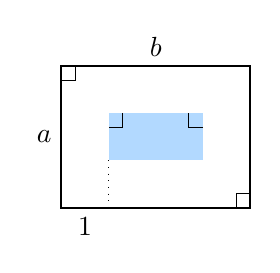
\begin{tikzpicture}[scale=0.6]
    \coordinate (A) at (0,0);
    \coordinate (B) at (4, 0);
    \coordinate (C) at (4, 3);
    \coordinate (D) at (0, 3);
    \coordinate (E) at (1, 1);
    \coordinate (F) at (1, 2);
    \coordinate (G) at (3, 2);
    \coordinate (H) at (3, 1);
    \coordinate (I) at (1, 0);

    \draw[thick] (A) -- (B) -- (C) -- (D) -- cycle;

    \fill[blue!50!cyan, opacity=0.3] (E) -- (F)-- (G)-- (H);
    \draw[dotted] (E) -- (I);

    \node[below] at ($(A)!0.5!(I)$) {$1$};
    \node[above] at ($(C)!0.5!(D)$) {$b$};
    \node[left] at ($(A)!0.5!(D)$) {$a$};

    \draw (F) ++(0.3,0) -- ++(0,-0.3) -- ++(-0.3,0);
    \draw (G) ++(0,-0.3) -- ++(-0.3,0) -- ++(0,0.3);
    \draw (B) ++(0,0.3) -- ++(-0.3,0) -- ++(0,-0.3);
    \draw (D) ++(0.3,0) -- ++(0,-0.3) -- ++(-0.3,0);
\end{tikzpicture}
\end{center}
Writing the equation,
\begin{align*}
    (a - 2)(b - 2) &= \frac{1}{2}ab \\
    2ab - 4a - 4b + 8 &= ab \\
    (a - 4)(b - 4) &= 8
\end{align*}
Notice that $a$ and $b$ are positive integers.
Therefore, there exists $\boxed{\text{two}}$ order pairs
$(3, 10)$ and $(4, 6)$ that satisfy the condition.
\end{solution}

\section*{\textcolor{BrickRed}{Challenge Problems}}
\subsection*{Problem}
The integer $N$ is positive. There are exactly $2005$
ordered pairs $(x, y)$ of positive integers satisfying:
\[
\frac{1}{x} + \frac{1}{y} = \frac{1}{N}
\]
Prove that $N$ is a perfect square.
\begin{proof}
First and foremost, rearrange the terms.
\begin{align*}
    \frac{1}{x} + \frac{1}{y} &= \frac{1}{N} \\
    \frac{x + y}{xy} &= \frac{1}{N} \\
    N(x + y) &= xy \\
    (x - N)(y - N) &= N^2
\end{align*}
Notice that because $x - N$ and $y - N$ are reflective,
the number of ordered pairs $(x, y)$ must be even,
unless there is a double counting. Double counting
only occurs when $x - N = y - N$. In other words,
there must be a factor $p$ where $p^2 = N$ for there
to be an odd number of ordered pairs.
\end{proof}

\subsection*{Problem}
$m$, $n$ are integers such that
\[
m^2 + 3m^2n^2 = 30n^2 + 517.
\]
Find $3m^2n^2$.

\begin{solution}
Simon's favorite factorization could be utilized.
\begin{align*}
    3m^2n^2 + m^2 - 30n^2 - 517 &= 0 \\
    (m^2 - 10)(3n^2 + 1) &= 507 = 3 \cdot 13^2
\end{align*}
Because $m$ and $n$ are integers, $m^2 - 10$ must be
$39$ while $3n^2 + 1$ is $13$. Therefore,
$49 \cdot 12 = \boxed{588}$.
\end{solution}

\subsection*{Problem}
There are two consecutive whole numbers such that
the difference of their cubes is equal to $181$ squared.
Find the sum of these two numbers.

\begin{solution}
Let the two consecutive whole numbers be $a$ and $a + 1$.
\begin{align*}
    (a + 1)^3 - a^3 &= 181^2 \\
    3a^2 + 3a + 1 &= 181^2 \\
    3a^2 + 3a &= 182 \cdot 180 \\
    a^2 + a - 182 \cdot 60 &= 0 \\
    a^2 + a - 10920 &= 0 \\
    100 < \sqrt{10920} &< 105 \\
    10920 &= 104 \cdot 105 \\
    (a + 105)(a - 104) &= 0
\end{align*}
Because $a$ is a whole number, $a = 104$.
Therefore, $104 + 105 = \boxed{209}$.
\end{solution}

\section*{Problem}
There exist unique positive integers $x$ and $y$ that
satisfy the equation $x^2 + 84x + 2008 = y^2$. Find $x + y$.

\begin{solution}
\begin{align*}
    x^2 + 84x + 1764 + 244 &= y^2 \\
    (x + 42)^2 + 244 &= y^2 \\
    (x + y + 42)(x - y + 42) &= -244
\end{align*}
Notice that $y$ must be greater than $x + 42$.
Moreover, $x + y + 42 = 122$ and $x - y + 42 = -2$
is a reasonable approach. Other cases does not work
because $x$ and $y$ are not natural numbers. Therefore,
$y = 62$ and $x = 18$. Thus, $x + y = \boxed{80}$.
\end{solution}
\end{document}

